\chapter{Beyond the Buzzwords: What AI Actually Means for Your Business}

\epigraph{The greatest enemy of knowledge is not ignorance, it is the illusion of knowledge.}{Stephen Hawking}

\section{A Brief History: From Mechanical Computation to Generative AI}

To understand why AI is suddenly everywhere, it helps to know where it came from. The story spans decades and involves surprising dead ends, unexpected breakthroughs, and a fundamental shift in what became possible.

\subsection{The Birth of Computers (1930s–1950s)}

Computers were not invented to do AI. They were invented to do math faster. In the 1930s, mathematicians and engineers asked a simple question: could a machine follow logical rules to solve problems? Alan Turing posed this in a theoretical way. John Atanasoff and Clifford Berry built the first electronic computer. By the 1940s, ENIAC (Electronic Numerical Integrator and Computer) was performing calculations for military purposes that would have taken human ``computers'' (actual people performing calculations) weeks.

The inventors had no grand vision of machines thinking like humans. They wanted to solve ballistics equations and break encryption codes. Computers were expensive, room-sized, and specialized tools.

Yet embedded in the question ``Can a machine follow logical rules?'' was the seed of something bigger: if a machine can follow rules, could it follow rules about thinking itself?

\subsection{Early AI Dreams (1956–1974)}

In 1956, a small group of researchers at Dartmouth College organized a summer workshop. They believed that human intelligence could be described precisely enough that machines could replicate it. They called it ``Artificial Intelligence.'' The optimism was breathtaking.

Over the next two decades, researchers built systems that could:

\begin{itemize}
\item Play checkers and chess by searching through possible moves
\item Solve mathematical problems through symbolic reasoning
\item Understand simple sentences by parsing grammar rules
\end{itemize}

These were impressive, and the field attracted significant government funding. The dream seemed within reach: if machines could search through logical possibilities faster than humans, maybe they could think faster too.

But by the mid-1970s, reality collided with promise. Chess-playing programs could beat amateurs but not grandmasters. Language understanding systems broke down on any sentence that deviated from narrow training. The problems turned out to be harder than anyone expected. Governments cut funding. The AI winter had begun.

\begin{keyinsight}
The first AI winter teaches an important lesson: enthusiasm without capability is expensive. Executives promised more than researchers could deliver. When the gap between hype and results became undeniable, funding dried up for nearly a decade.
\end{keyinsight}

\subsection{The AI Comeback: Machine Learning and Expert Systems (1980s–1990s)}

By the 1980s, a different approach emerged. Instead of trying to encode human knowledge into logical rules, researchers began building systems that learned patterns from data. This was machine learning.

Expert systems became the first commercial success. They encoded the knowledge of human experts (a radiologist, a mechanic, a financial analyst) into decision rules. A bank could deploy a system trained on thousands of loan decisions to automatically evaluate new applications. An insurance company could use a system trained on repair histories to estimate claim costs. These systems worked---not perfectly, but well enough to create business value.

But they remained narrow. An expert system trained on loan approvals could not help with insurance claims. It could not transfer what it ``learned'' (really, what humans programmed it to know) to new domains.

\subsection{The Internet and Data Explosion (1990s–2010s)}

The internet changed the game. Suddenly, companies had access to massive amounts of data: user behavior (clickstreams), customer feedback (reviews), transaction records, sensor data from IoT devices. Machine learning algorithms thrived on data.

By the 2000s, AI was everywhere---though most people did not call it that:

\begin{itemize}
\item \textbf{Search engines} ranked pages using machine learning algorithms trained on billions of examples of good vs. bad search results.
\item \textbf{Recommendation systems} at Netflix and Amazon learned which shows and products users liked by observing their behavior.
\item \textbf{Spam filters} classified incoming emails by learning patterns from millions of examples of spam and legitimate mail.
\item \textbf{Credit scoring and fraud detection} flagged unusual transactions using systems trained on historical data.
\item \textbf{Mobile phones} learned faces (facial recognition) and understood spoken commands (voice recognition) using deep neural networks.
\end{itemize}

These systems were not called ``AI'' in marketing---they were features. But they were machine learning, and they worked. Companies competing on these systems had massive advantages. Google's ranking algorithm was more valuable than any physical asset.

The term ``AI'' fell out of fashion because it was too loaded with hype and unfulfilled promises. Engineers simply said ``machine learning'' or ``data science'' and got on with building valuable systems.

\subsection{Deep Learning and Modern AI (2012–2021)}

In 2012, a computer vision system trained on deep neural networks dramatically outperformed traditional methods at recognizing objects in images. Deep learning had arrived.

For the next decade, deep learning systems drove breakthroughs:

\begin{itemize}
\item \textbf{Computer vision} systems could identify people, objects, and scenes almost as well as humans.
\item \textbf{Natural language processing} could translate between languages, understand sentiment in text, and generate plausible (if repetitive) responses.
\item \textbf{Speech recognition} became accurate enough for virtual assistants and real-time transcription.
\item \textbf{Game-playing systems} defeated world champions in chess, Go, and competitive video games.
\end{itemize}

Companies like Google, Facebook, and Amazon built enormous AI research teams. Startups raised billions on the premise that AI would transform every industry. Yet for most businesses and employees, the impact was still hidden or indirect. AI was a backend technology driving features you used without thinking about it.

The big breakthrough---language models that could engage in extended conversation---was coming, but not quite yet.

\subsection{The Generative AI Leap (2022–Present)}

In November 2022, OpenAI released ChatGPT. Within two months, it had one hundred million users---faster adoption than any consumer application in history.

Why the sudden shift? Three ingredients aligned:

\begin{enumerate}
\item \textbf{Scale:} Language models trained on hundreds of billions of words could capture patterns that smaller models missed. When you scale up the data and compute, something changes---qualitatively.
\item \textbf{Instruction tuning:} Researchers figured out how to train models to follow instructions and generate coherent multi-paragraph responses, not just complete sentences.
\item \textbf{Accessible interface:} ChatGPT was not a research paper or a specialized tool. Anyone with a web browser could interact with it in plain English.
\end{enumerate}

Suddenly, a tool could write emails, draft reports, debug code, and explain concepts---and do it well enough to be immediately useful. The leap was not purely technical (researchers had the fundamentals) but practical: these models became tools people could actually use.

What changed is not just capability. It is accessibility. For the first time, powerful AI did not require data science expertise, massive infrastructure investment, or years of custom development. It was available to anyone with a prompt.

\begin{realexample}[The Difference GenAI Made]
A management consulting firm spent 2019–2022 building an internal tool to generate client presentations. It required a dedicated data science team, cost millions in development, and worked only for standardized presentations.

In late 2022, junior consultants started using ChatGPT to draft presentation decks. Within weeks, the tool was unofficially in use across the firm. The expensive internal system was quietly retired. The results were not always perfect, but they were fast and cheap. The firm repurposed the data science team to higher-value work.

This story repeated across thousands of organizations in 2023–2024.
\end{realexample}

\subsection{Why This Time Is Different}

Throughout the history of AI, there was always a gap between capability and access. In the 1950s, only researchers with access to million-dollar computers could do AI research. In the 1990s, you needed a data science team and years of development. Even in 2020, building a working recommendation system or chatbot required significant expertise and infrastructure.

That gap has closed. Today, a high school student can use GPT-4 to draft a research paper. A small business owner can use Claude to analyze customer feedback. A sales team can use Copilot to draft proposals. No PhD required. No infrastructure investment required.

This is not the first time AI promised to transform everything. But it is the first time the tools are accessible enough, capable enough, and integrated into everyday workflows that the adoption curve looks different. The chicken-and-egg problem is solved: you do not need to implement a huge AI project to see value. You can start with a prompt.

\section{The Many Meanings of ``AI''}

Every quarter, someone walks into a board meeting with a slide deck featuring ``AI-powered'' solutions. The term has been stretched to cover everything from spam filters to autonomous vehicles. This creates confusion---and confusion is expensive.

When a vendor says ``AI-powered,'' they might mean rule-based systems that follow explicit if-then logic (traditional software, not really AI in the modern sense), or machine learning systems that learn patterns from data to make predictions. They might mean deep learning, which uses neural networks to handle complex patterns in images and language. Or they might mean generative AI---systems that create new content like text, images, and audio.

These categories nest inside each other like Russian dolls. All generative AI uses deep learning, all deep learning is machine learning, and all machine learning falls under the broad umbrella of artificial intelligence. But the capabilities and business applications differ dramatically at each level.

For this book, we focus primarily on generative AI and its practical business applications, because that is where the immediate opportunities lie for most executives. When you hear about ChatGPT, Claude, Copilot, or similar tools at industry conferences, you are hearing about generative AI.

\begin{figure}[htbp]
\centering
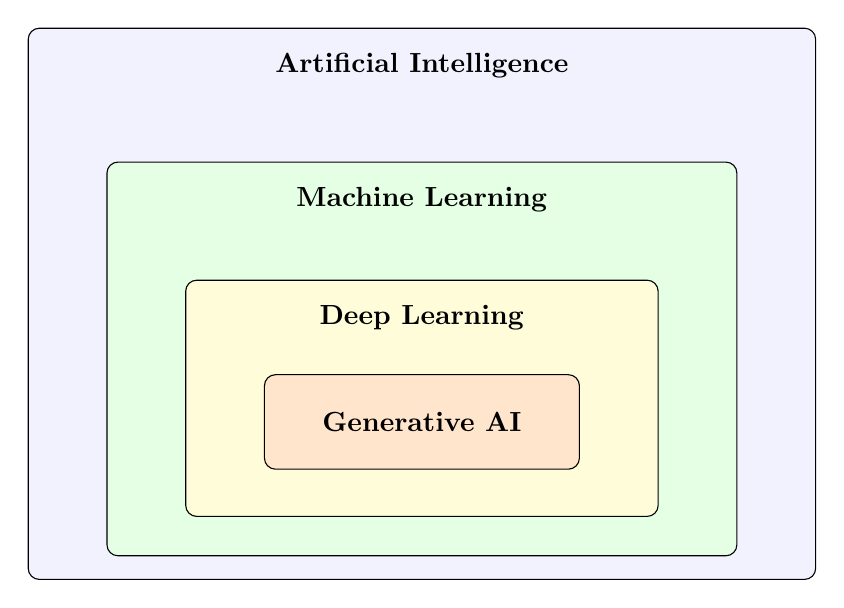
\begin{tikzpicture}
    % Outermost box - AI
    \node[draw, rounded corners, minimum width=10cm, minimum height=7cm, fill=blue!5] (ai) {};
    \node[anchor=north] at ([yshift=-0.2cm]ai.north) {\textbf{Artificial Intelligence}};

    % Machine Learning box
    \node[draw, rounded corners, minimum width=8cm, minimum height=5cm, fill=green!10] at ([yshift=-0.7cm]ai.center) (ml) {};
    \node[anchor=north] at ([yshift=-0.2cm]ml.north) {\textbf{Machine Learning}};

    % Deep Learning box
    \node[draw, rounded corners, minimum width=6cm, minimum height=3cm, fill=yellow!15] at ([yshift=-0.5cm]ml.center) (dl) {};
    \node[anchor=north] at ([yshift=-0.2cm]dl.north) {\textbf{Deep Learning}};

    % Generative AI box
    \node[draw, rounded corners, minimum width=4cm, minimum height=1.2cm, fill=orange!20] at ([yshift=-0.3cm]dl.center) (gen) {};
    \node at (gen.center) {\textbf{Generative AI}};
\end{tikzpicture}
\caption{The relationship between AI, machine learning, deep learning, and generative AI}
\label{fig:ai-hierarchy}
\end{figure}

\section{From Rules to Predictions: A Fundamental Business Shift}

Traditional business software follows rules: ``If customer spent over \$1000, offer 10\% discount.'' Someone on your team defined that rule. The software executes it.

AI systems work differently. You show them thousands of examples: customers who responded well to discounts, customers who did not. The system identifies patterns you never explicitly defined. Maybe it discovers that customers who browse on mobile devices on Sunday evenings respond better to free shipping than percentage discounts---an insight no analyst thought to look for.

This shift from ``rules we write'' to ``patterns the system discovers'' is the core mental model to understand. It changes how you think about business process optimization, customer insights, and competitive intelligence.

\begin{table}[htbp]
\centering
\begin{tabularx}{\textwidth}{lXX}
\toprule
\textbf{Aspect} & \textbf{Traditional Software} & \textbf{AI/ML Systems} \\
\midrule
Logic & Rules written by humans & Patterns learned from data \\
Changes & Requires code updates & Can adapt with new data \\
Predictions & Deterministic, same input = same output & Probabilistic, may vary \\
Edge cases & Must be explicitly handled & May generalize (or fail) \\
Explainability & Clear, traceable logic & Often opaque \\
\bottomrule
\end{tabularx}
\caption{Comparing traditional software and AI systems}
\end{table}

\section{What Generative AI Really Does}

Generative AI predicts what should come next.

When you ask ChatGPT a question, it is predicting: ``Given this question, what response would most likely follow based on billions of examples I learned from?'' It is not ``thinking'' or ``understanding'' in the human sense. It is sophisticated pattern matching at unprecedented scale.

This explains both its strengths and failures. It sounds fluent because it learned from fluent text. It can be confidently wrong because ``sounding right'' and ``being right'' are entirely different things. And it struggles with novel reasoning because it relies on patterns rather than genuine understanding.

\begin{keyinsight}
Think of generative AI as the world's most sophisticated autocomplete. It is remarkably good at predicting what text should come next based on patterns. But prediction is not understanding, and fluency is not accuracy. This distinction drives every decision about when to use AI and when to rely on human judgment.
\end{keyinsight}

\section{Where AI Is Already Around You}

Before you ``adopt AI,'' recognize you are already using it:

\begin{table}[htbp]
\centering
\begin{tabular}{ll}
\toprule
\textbf{Service} & \textbf{AI Application} \\
\midrule
Email spam filtering & Classification ML \\
Netflix recommendations & Recommendation systems \\
Google search results & Ranking algorithms + LLMs \\
Phone face unlock & Computer vision \\
Credit card fraud alerts & Anomaly detection \\
Autocorrect/autocomplete & Language models \\
\bottomrule
\end{tabular}
\caption{AI you already use daily}
\end{table}

The question is not whether to use AI---it is whether to use it more deliberately and strategically.

\section{Why This Time Is Different: The Business Case}

Previous AI hype cycles (2015, 2018) promised transformations that did not materialize for most businesses. Executives who ignored those waves often looked wise. This time is different, and here is why:

\textbf{Accessibility changed.} You no longer need a data science team to use AI. ChatGPT, Claude, and Copilot work through natural language. If you can describe what you want, you can use these tools. Your marketing director can use AI today---no IT ticket required.

\textbf{Capabilities crossed a threshold.} Pre-2022 language models were interesting but not business-ready. Current models can draft contracts, analyze financial reports, prepare board presentations, and summarize complex documents at a level that is genuinely useful.

\textbf{Cost dropped dramatically.} What cost thousands in computing three years ago now costs pennies per task. The unit economics changed fundamentally.

\textbf{The competitive pressure is real.} Your competitors are using these tools. The productivity gap between AI-assisted and non-AI-assisted work is widening. Early adopters are pulling ahead in operational efficiency.

\begin{realexample}[The Productivity Gap]
A professional services firm tracked two teams doing similar client analysis work. The team using AI tools consistently delivered reports 40\% faster with comparable quality. After six months, the difference in client capacity was significant. The AI-assisted team could handle more engagements, leading to higher revenue per consultant and better client satisfaction scores. The firm is now rolling out AI tools company-wide.
\end{realexample}

\section{What This Book Will and Will Not Cover}

This book focuses on practical application. You will learn how to use existing AI tools effectively---ChatGPT, Claude, Copilot, and specialized industry tools---along with frameworks for evaluating when AI is appropriate for a given task. We will cover managing AI risks around accuracy, privacy, and bias, implementing concrete projects with measurable results, and building organizational capability over time.

What we will not cover: building custom AI models from scratch, technical machine learning theory, AI for highly specialized domains like medical diagnosis or autonomous vehicles, or speculation about future capabilities that do not yet exist. This is a book about using AI as it exists today to solve business problems you face now.

\section{Summary}

AI is not magic. It is a set of prediction and pattern-recognition tools that turn data into useful business outputs. Generative AI creates new content---text, analysis, presentations---from patterns it has learned.

The shift from rule-based software to pattern-based AI represents a fundamental change in how businesses can operate. But leveraging this shift requires knowing both what AI does well and where it fails.

You are already using AI every day, whether you realize it or not. The strategic question now is whether to use it more deliberately, more systematically, and more competitively. That starts with understanding how AI systems actually ``think''---which is the subject of our next chapter.

\begin{exercise}
List five AI-powered services you use in a typical week. For each, identify what the AI is actually doing (classification, prediction, generation, recommendation).
\end{exercise}

\begin{exercise}
Find three ``AI-powered'' products in your industry. Research what kind of AI they actually use. Are they using generative AI, machine learning for predictions, or something else?
\end{exercise}
